\documentclass{article}

\usepackage[heading=true]{ctex}
\usepackage[backref]{hyperref}
\usepackage{amsmath}
\usepackage{filecontents}
\usepackage{float}
\usepackage{graphicx}
\usepackage{geometry}
\usepackage{dirtree}
\usepackage{listings}
\usepackage{xcolor}
\usepackage{qtree}

\ctexset{
    section={
        number=\chinese{section},
        format+=\raggedright
    }
}
\geometry{a4paper, scale=0.7}

\title{实验四: RNN、GRU、LSTM和Bi-LSTM}
\author{1190200703 管健男}
\date{}

\begin{document}
\maketitle

\section{模型结构}

根据以下模型结构和公式,即可利用pytorch内置的函数搭建出相应的模型。

\subsection{RNN}

RNN结构如图\ref{RNN}。

\begin{figure}[H]
    \centering
    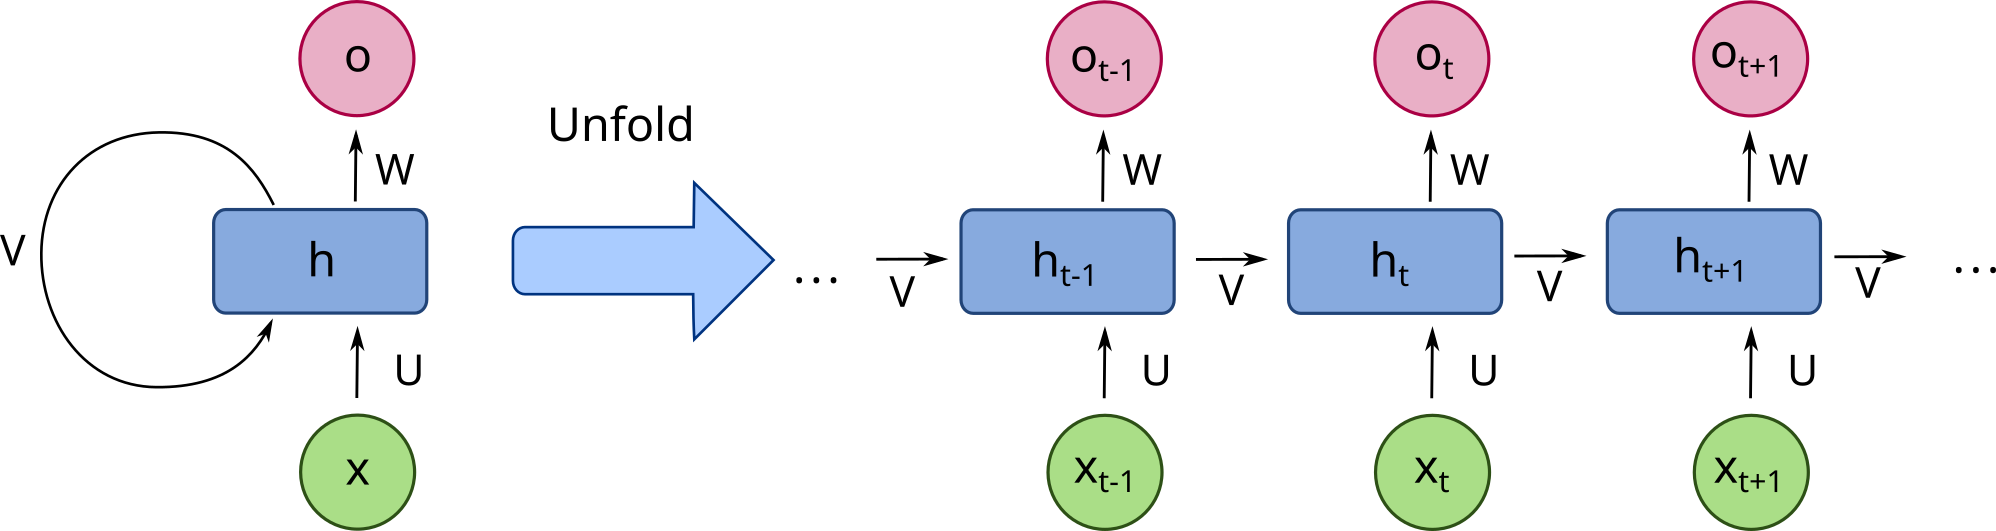
\includegraphics[width=0.8\textwidth]{figures/rnn.png}
    \caption{RNN结构}
    \label{RNN}
\end{figure}

用公式表示如下:

\begin{gather*}
    h_t = f(U X_t + W h_{t-1}) \\
    O_t = g(V h_t)
\end{gather*}

对于文本分类这个N to 1问题,需要在最后一个$O_t$之后加一层softmax输出各个类别的概率。

\subsection{GRU}

GRU结构如图\ref{GRU}。

\begin{figure}[H]
    \centering
    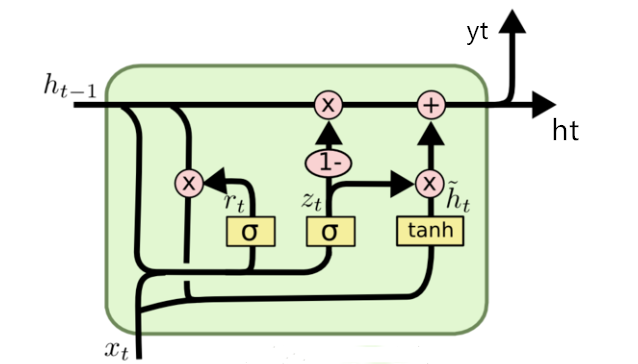
\includegraphics[width=0.5\textwidth]{figures/gru.png}
    \caption{GRU结构}
    \label{GRU}
\end{figure}

用公式表示如下:

\begin{gather*}
    z_t = \sigma_g(W_z x_t + U_z h_{t-1} + b_z) \\
    r_t = \sigma_g(W_r x_t + U_r h_{t-1} + b_r) \\
    \hat{h}_t = \phi_h\left(W_h x_t + U_h (t_t \odot h_{t-1}) + b_r\right) \\
    h_t = z_t \odot \hat{h}_t + (1 - z_t) \odot h_{t-1}
\end{gather*}

\subsection{LSTM}

LSTM结构如图\ref{LSTM}。

\begin{figure}[H]
    \centering
    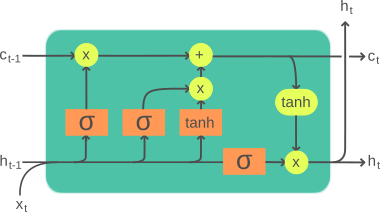
\includegraphics[width=0.5\textwidth]{figures/lstm.png}
    \caption{LSTM结构}
    \label{LSTM}
\end{figure}

用公式表示如下:

\begin{gather*}
    f_t = \sigma_g(W_f x_t + U_f h_{t-1} + b_f) \\
    i_t = \sigma_g(W_i x_t + U_i h_{t-1} + b_i) \\
    o_t = \sigma_g(W_o x_t + U_o h_{t-1} + b_o) \\
    \hat{c}_t = \sigma_c(W_c x_t + U_c h_{t-1} + b_c) \\
    c_t = f_t \circ c_{t-1} + i_t \circ \hat{c}_t \\
    h_t = o_t \circ \sigma_t(c_t)
\end{gather*}

\subsection{BiLSTM}

BiLSTM结构如图\ref{BiLSTM}。

\begin{figure}[H]
    \centering
    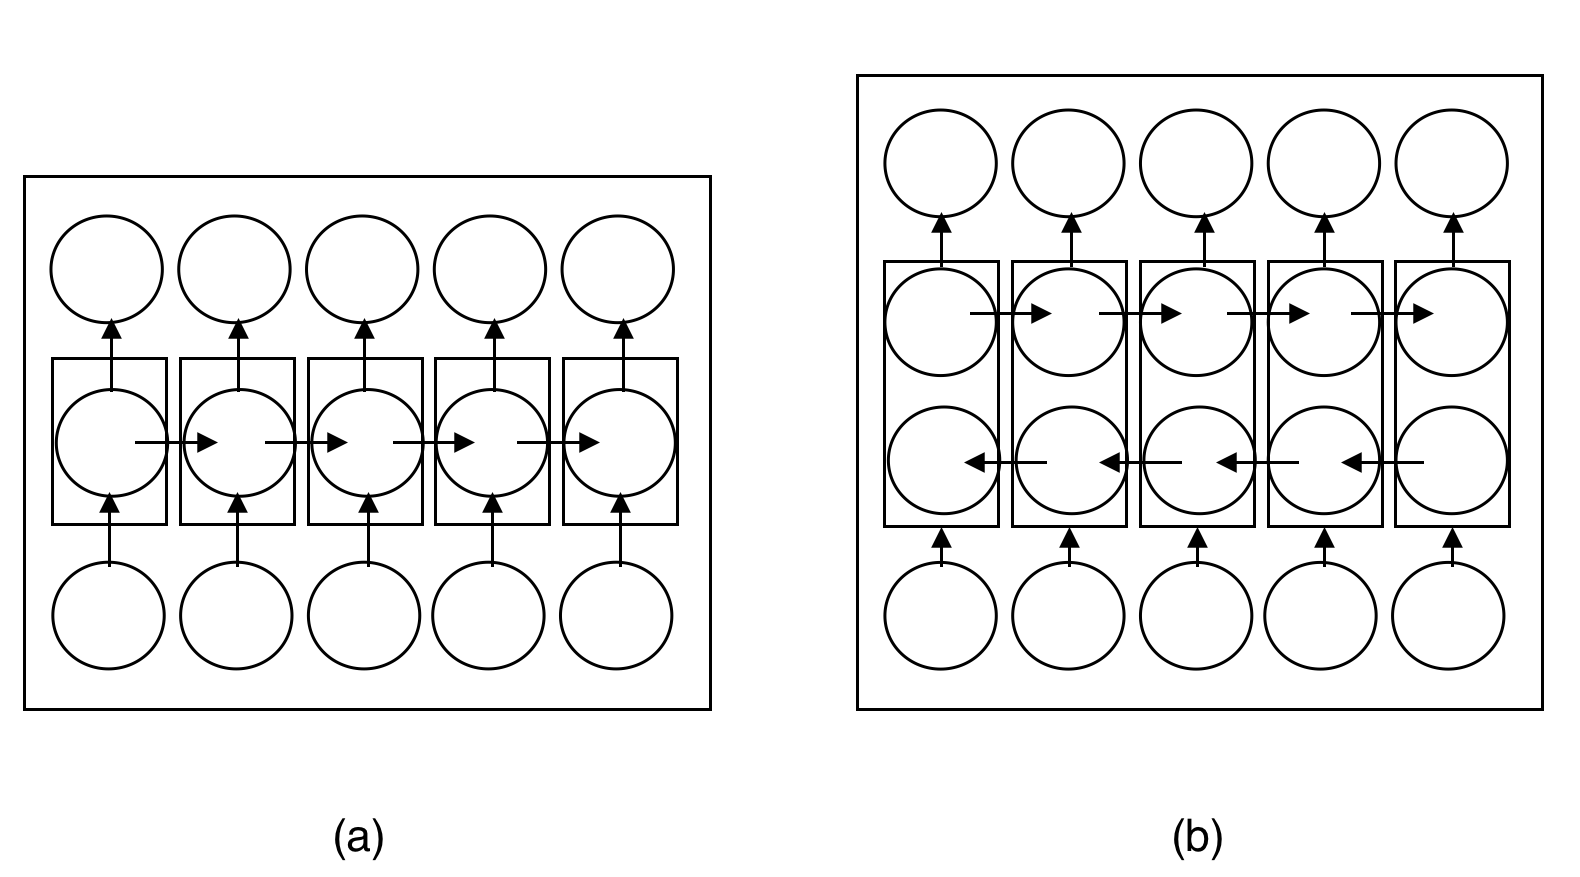
\includegraphics[width=0.7\textwidth]{figures/bilstm.png}
    \caption{BiLSTM结构}
    \label{BiLSTM}
\end{figure}

基本原理和LSTM相同,但是相当于两个LSTM的复合:
一个接受输入并向前传递,另一个接受输入并向后传递。

\section{文本多分类任务}

\subsection{模型结果}

利用上述四种结构进行文本多分类计算测试结果的F1值,
如表\ref{result-text}所示。

\begin{table}[h]
    \centering
    \begin{tabular}{lll}
        \hline
        \textbf{Model} & \textbf{micro F1} & \textbf{macro F1} \\
        \hline
        \hline
        RNN            & 69.930\%          & 51.141\%          \\
        GRU            & 76.294\%          & 49.933\%          \\
        LSTM           & 82.308\%          & 67.288\%          \\
        BiLSTM         & 87.167\%          & 79.030\%          \\
        \hline
    \end{tabular}
    \label{result-text}
    \caption{四种模型结构进行文本多分类的测试结果的F1值}
\end{table}

四种模型的micro F1值和macro F1的在训练过程中的变化如图\ref{mif1}和\ref{maf1}所示。

\begin{figure}[H]
    \centering
    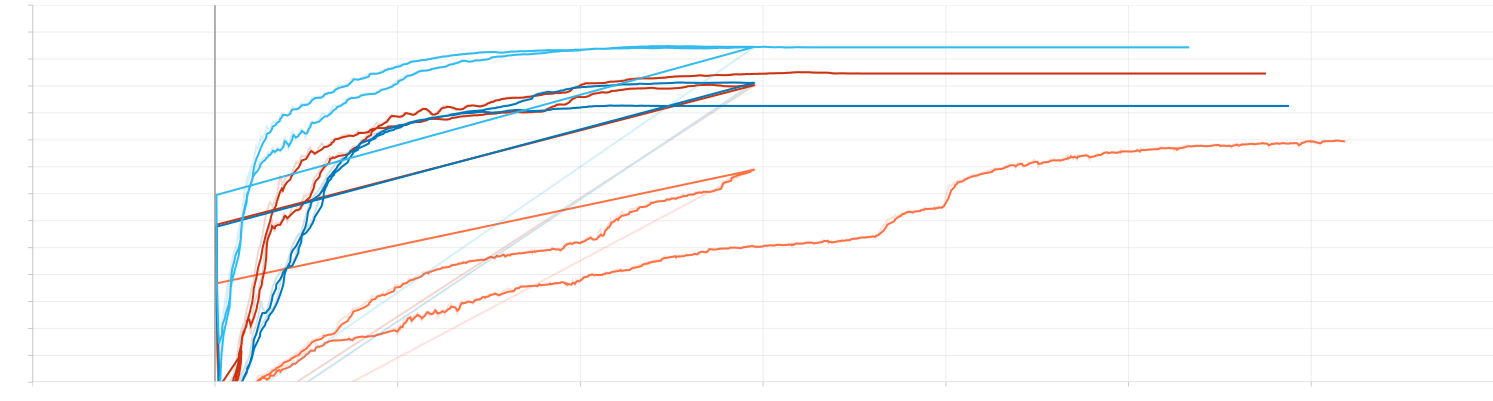
\includegraphics[width=0.8\textwidth]{figures/MicroF1Score_dev.png}
    \caption{四种模型的micro F1值的变化}
    \label{mif1}
\end{figure}

\begin{figure}[H]
    \centering
    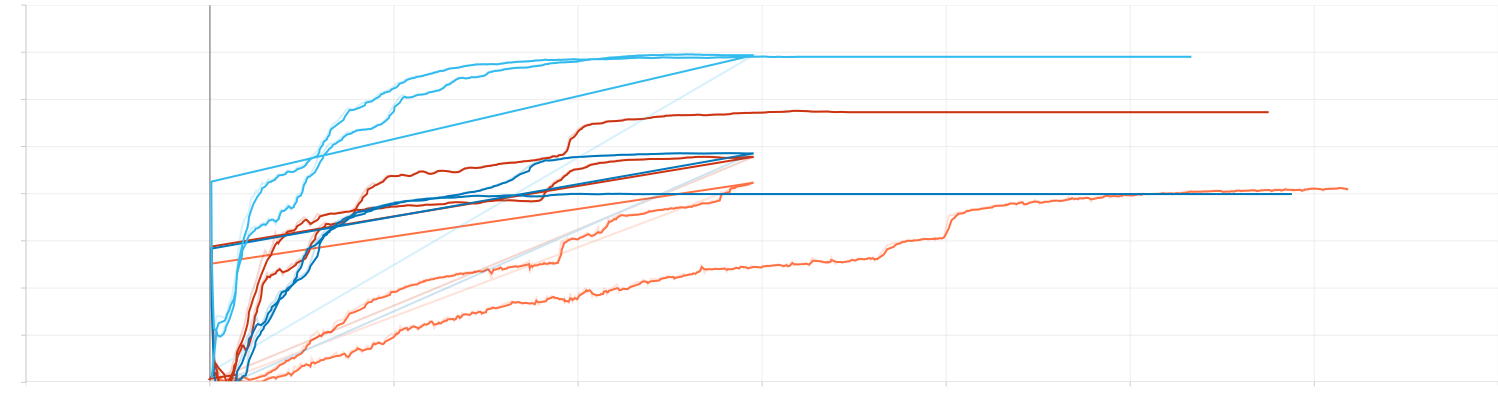
\includegraphics[width=0.8\textwidth]{figures/MacroF1Score_dev.png}
    \caption{四种模型的macro F1值的变化}
    \label{maf1}
\end{figure}

\subsection{结果分析}

对比分析四种结构的实验结果,可以看到 BiLSTM 性能最好,LSTM 次之,
GRU 的 micro F1 优于 RNN 但是 macro F1 略逊于 RNN。

\subsection{经验总结}

在实际训练时发现,由于RNN和GRU的记忆能力并不算强,
因此每句话的长度应该裁剪或填充到一个不太大的值,否则模型效率将减弱很多。
而LSTM和BiLSTM的记忆能力允许他们接受一个更长的句子作为输入。
在本次实验中,RNN和GRU的句子长度都设置为了64,
而LSTM和BiLSTM的句子长度是128。

\section{温度预测}

\subsection{模型结果}

使用LSTM进行温度预测,由于天气具有较大的不确定性,所以仍然有预测不准的情况。

预测比较准的情况如图\ref{weather-good1}

\begin{figure}[H]
    \centering
    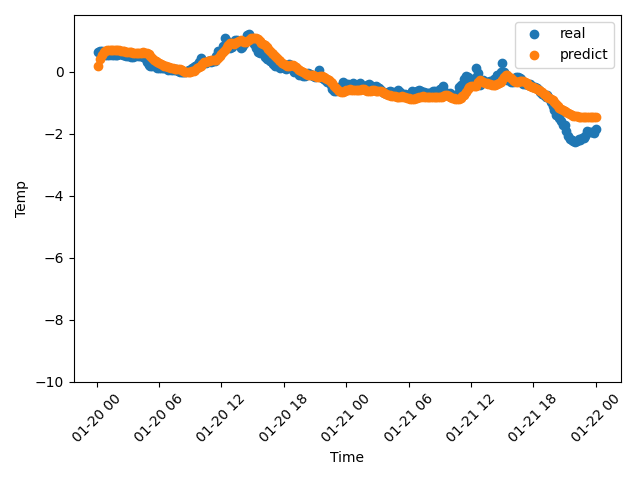
\includegraphics[width=0.5\textwidth]{figures/weather_good1.png}
    \caption{预测较准的情况}
    \label{weather-good1}
\end{figure}

预测一般的情况如图\ref{weather-mid1}。

\begin{figure}[H]
    \begin{minipage}[H]{0.3\linewidth}
        \centering
        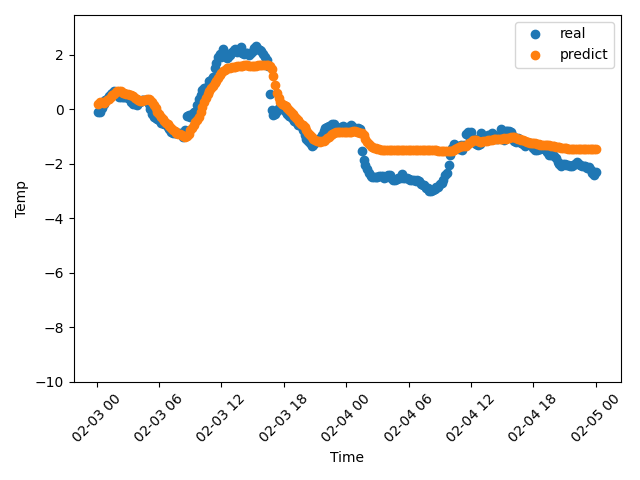
\includegraphics[width=\textwidth]{figures/weather_mid1.png}
    \end{minipage}
    \begin{minipage}[H]{0.3\linewidth}
        \centering
        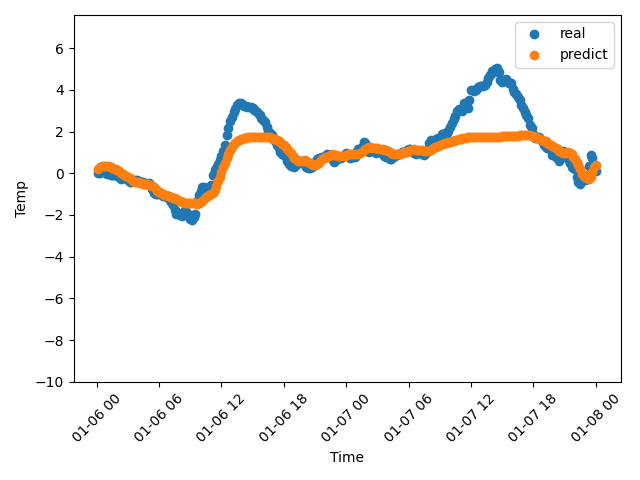
\includegraphics[width=\textwidth]{figures/weather_mid2.png}
    \end{minipage}
    \begin{minipage}[H]{0.3\linewidth}
        \centering
        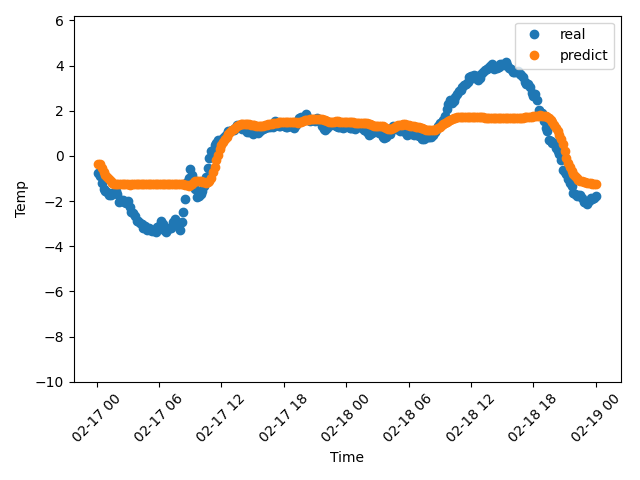
\includegraphics[width=\textwidth]{figures/weather_mid3.png}
    \end{minipage}
    \caption{预测一般的情况}
    \label{weather-mid1}
\end{figure}

预测比较差的情况如图\ref{weather-bad1}。

\begin{figure}[H]
    \centering
    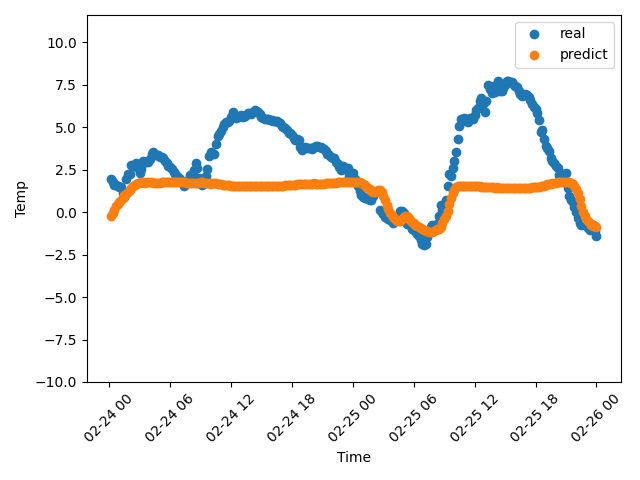
\includegraphics[width=0.5\textwidth]{figures/weather_bad1.png}
    \caption{预测一般的情况}
    \label{weather-bad1}
\end{figure}

MAE和MSE分别如图\ref{mae}和\ref{mse}。

\begin{figure}[H]
    \centering
    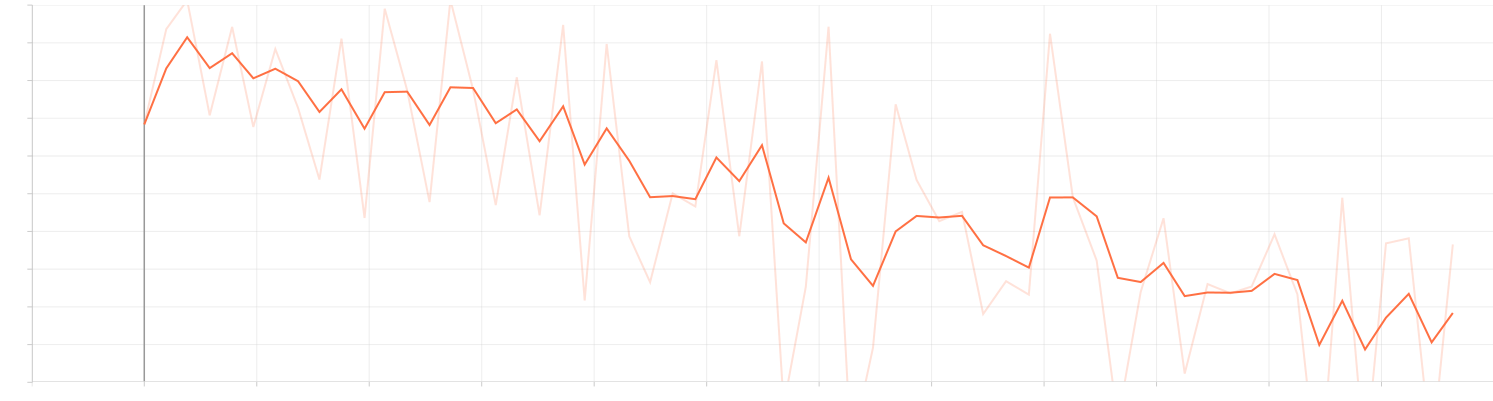
\includegraphics[width=0.8\textwidth]{figures/mae.png}
    \caption{MAE}
    \label{mae}
\end{figure}

\begin{figure}[H]
    \centering
    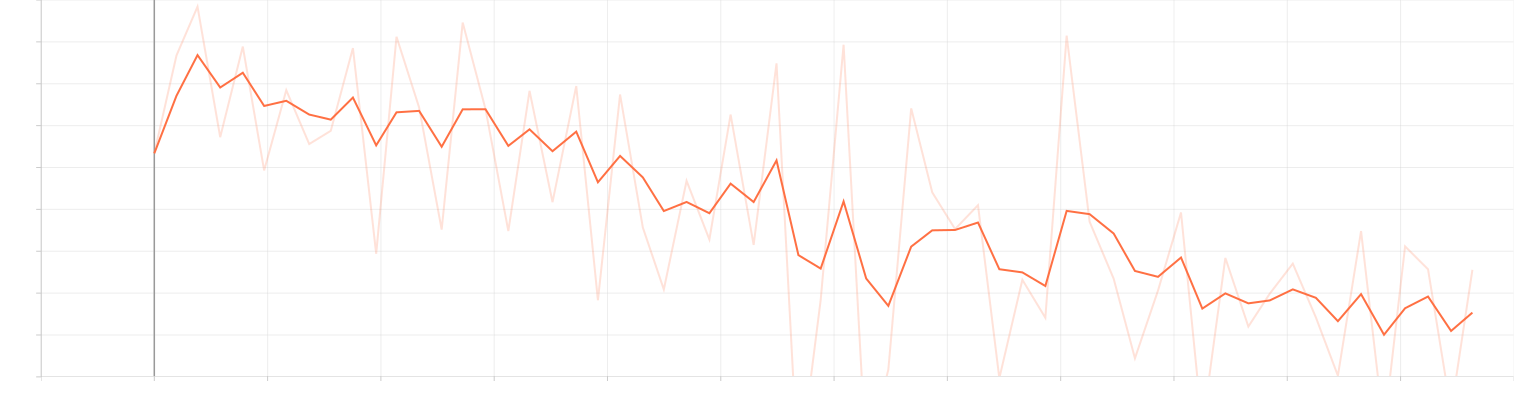
\includegraphics[width=0.8\textwidth]{figures/mse.png}
    \caption{MSE}
    \label{mse}
\end{figure}

最佳的MAE和MSE如表\ref{maemse}。

\begin{table}[h]
    \centering
    \begin{tabular}{lll}
        \hline
        \textbf{MAE} & \textbf{MSE} \\
        \hline
        9.53         & 137.78       \\
        \hline
    \end{tabular}
    \label{maemse}
    \caption{MAE和MSE}
\end{table}

\end{document}
